\documentclass[border=2pt]{standalone}
\usepackage{tikz}
\usetikzlibrary{datavisualization.formats.functions,datavisualization.polar}
\begin{document}
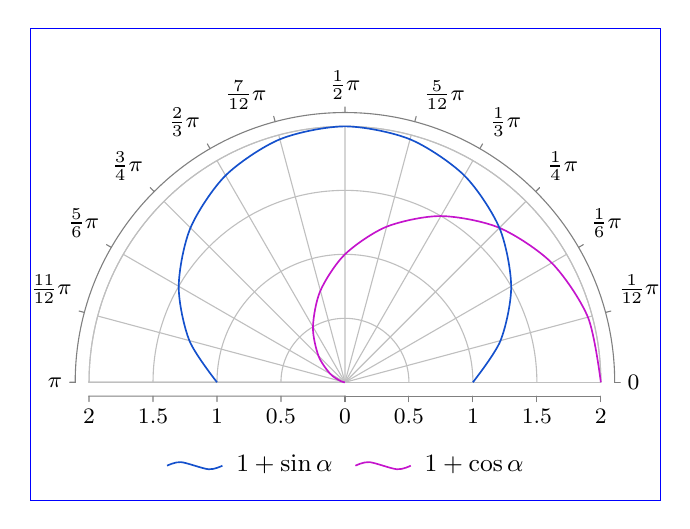
\begin{tikzpicture}
  \draw[blue,line width=.2pt] (-4,-1.5) rectangle (4,4.5);
  \datavisualization [scientific polar axes={0 to pi,clean},all axes=grid,
    style sheet=vary hue,legend=below]
    [visualize as smooth line=sin,sin={label in legend={text=$1+\sin\alpha$}}]
    data [format=function] {
      var angle : interval [0:pi] samples 13;
      func radius = sin(\value{angle}r) + 1;
    }
    [visualize as smooth line=cos,cos={label in legend={text=$1+\cos\alpha$}}]
    data [format=function] {
      var angle : interval [0:pi] samples 13;
      func radius = cos(\value{angle}r) + 1;
    };
\end{tikzpicture}
\end{document}
